% =============================================================================
%  Two-Mode Active-Subspace Reduction and Reciprocal Determinant Thresholds
%  in Linear Ornstein-Uhlenbeck Systems
%
%  FIRST DRAFT -- September 2026.  Not deposited, not submitted.
%
%  Self-contained: main.tex + references.bib + figures/ in this directory.
%  Build:  ./build.sh      (latexmk -pdf, or pdflatex/bibtex/pdflatex x2)
%  Checks: python3 manuscript_checks.py   (55 exact symbolic checks)
% =============================================================================

\documentclass[11pt]{article}

\usepackage[letterpaper,margin=1in]{geometry}
\usepackage{amsmath,amssymb,amsthm}
\usepackage{graphicx}
\usepackage{booktabs}
\usepackage[T1]{fontenc}
\usepackage[utf8]{inputenc}
\usepackage{microtype}
\usepackage[colorlinks=true,linkcolor=blue,citecolor=blue,urlcolor=blue]{hyperref}

\theoremstyle{plain}
\newtheorem{theorem}{Theorem}
\newtheorem{proposition}[theorem]{Proposition}
\newtheorem{lemma}[theorem]{Lemma}
\newtheorem{corollary}[theorem]{Corollary}
\theoremstyle{definition}
\newtheorem{definition}[theorem]{Definition}
\theoremstyle{remark}
\newtheorem{remark}[theorem]{Remark}

\newcommand{\tr}{\operatorname{tr}}
\newcommand{\Real}{\mathbb{R}}
\newcommand{\Sig}{\Sigma}
\newcommand{\Aco}{\mathcal{A}}
\newcommand{\eperp}{e^{\perp}}
\newcommand{\eperpT}{e^{\perp\!\top}}
\newcommand{\T}{^{\!\top}}

\title{Two-Mode Active-Subspace Reduction and\\
Reciprocal Determinant Thresholds in\\
Linear Ornstein--Uhlenbeck Systems}
\author{Elias De Jes\'us\\
Independent Researcher\\
ORCID: 0009-0007-0190-9143}
\date{First draft --- September 2026}

\begin{document}
\maketitle

\begin{abstract}
We study the stationary covariance of a stable linear Ornstein--Uhlenbeck system whose drift,
restricted to a two-dimensional invariant subspace, has distinct relaxation rates $D_1,D_2>0$,
and whose forcing on that subspace is a rank-one deformation of an isotropic baseline,
$Q=q_b\bigl(I+(\tau-1)ee\T\bigr)$, along a unit \emph{excitation direction} $e=cu+sv$. Here
$\tau>0$ is a \emph{variance} ratio. Solving the Lyapunov equation on the plane gives an exact
$2\times2$ block, and we prove that its determinant is an exactly \emph{palindromic} quadratic
in $\tau$:
\[
  4D_1D_2\det\Sig = q_b^2\bigl(\Aco\tau^2+(1-2\Aco)\tau+\Aco\bigr),
  \qquad \Aco=c^2s^2\nu^2,\quad \nu=\frac{D_1-D_2}{D_1+D_2}.
\]
The leading and constant coefficients coincide because the forcing family is self-dual,
$Q_e(\tau)=\tau\,Q_{\eperp}(1/\tau)$, which is $ee\T+\eperp\eperpT=I$ in disguise. Only then
does the reciprocal coordinate $w=\tau+1/\tau$ appear: dividing by $\tau$ makes the normalized
determinant exactly affine in $w$, which yields an exact generalized-variance threshold. The
coefficient $\Aco$ vanishes precisely when the excitation lies in a single drift eigenmode or
the two rates coincide, and is maximized at equal modal weights. Graph-Laplacian systems give
corollaries: the two-node model of earlier work is recovered with $\tau=r^2$, and $P_3$ and
$K_3$ give exact optimal thresholds $35+15\sqrt5$ and $247/2$. The central identities are
machine-checked in Lean~4 with mathlib. We emphasize that the one-coordinate closure is tied
to an effectively two-dimensional active structure and does not extend automatically to
genuinely multi-mode excitation.
\end{abstract}

\section{Introduction}\label{sec:intro}

Linear Ornstein--Uhlenbeck (OU) systems are among the few multivariate stochastic models whose
stationary statistics are available in closed form: for a Hurwitz drift the stationary
covariance solves an algebraic Lyapunov equation
\cite{UhlenbeckOrnstein1930,Gardiner2004,Vatiwutipong2019}. This makes them a natural setting in
which to ask how \emph{heterogeneous} forcing interacts with coupling, and the question has been
studied directly: Barucca analyses localization in covariance matrices of coupled heterogeneous
OU processes \cite{Barucca2014}; Ferreira, Metz and Barucca develop a random-matrix ensemble for
OU covariances with heterogeneous temperatures \cite{FerreiraMetzBarucca2025}; Godr\`eche and
Luck give exact nonequilibrium stationary states for linear Langevin systems at two temperatures
\cite{GodrecheLuck2019}; and the Brownian-gyrator literature studies the same two-temperature
structure in a planar model \cite{FilligerReimann2007,DotsenkoEtAl2013}.

A scalar summary of such a covariance is its determinant, Wilks's generalized variance
\cite{Wilks1932}, which is monotone in the differential entropy of the stationary Gaussian
\cite{CoverThomas2005}. Earlier work of the author \cite{DeJesus2026ou} analysed two diffusively
coupled OU processes with unequal noise amplitudes and found that this determinant can exceed
its uncoupled value at finite coupling if and only if the noise-amplitude ratio exceeds
$3+2\sqrt2$ --- an exact algebraic threshold in a two-node model.

The starting point of the present paper is that the two-node graph is \emph{not} the essential
structure. What matters is a geometric configuration that a two-node system happens to realize:
a two-dimensional invariant subspace of the drift on which the relaxation rates differ, carrying
a forcing that is isotropic except for a rank-one deformation along one direction. We call that
subspace the \emph{active plane} and that direction the \emph{excitation direction}. Under those
hypotheses --- and with no reference to any graph --- the stationary covariance determinant is
exactly palindromic in the variance ratio, and therefore collapses onto the single reciprocal
coordinate $w=\tau+1/\tau$.

The logical order matters and we keep it throughout. The reciprocal coordinate is not posited as
a convenient change of variable: it is \emph{forced} by an algebraic symmetry of the determinant,
which is in turn forced by a self-duality of the rank-one forcing family. The chain is
\[
\begin{gathered}
  \text{rank-one excitation}\ \to\ \text{two-mode covariance block}
  \ \to\ \text{palindromic determinant}\\
  \to\ w=\tau+1/\tau\ \to\ \text{exact threshold},
\end{gathered}
\]
and each arrow is proved before the next is used.

\paragraph{What is standard and what is not.} The ingredients are almost entirely classical: the
OU stationary covariance and the Lyapunov equation \cite{Gardiner2004}; the modal solution
$\Sig_{ij}=Q_{ij}/(D_i+D_j)$, standard in the heterogeneous-OU literature
\cite{Barucca2014,GodrecheLuck2019}; the reduction of a self-reciprocal polynomial through
$t+1/t$ \cite{Vieira2019}; the trace/determinant shape statistic and its relation to Mauchly's
sphericity test \cite{Mauchly1940,Muirhead1982}; and the Newton-identity obstruction in dimension
$n\ge3$. What we did not locate in the literature we searched is the specific assembly: the exact
palindromic determinant identity, its reciprocal reduction, and the resulting exact
generalized-variance threshold optimized over a coupling parameter. We state that conservatively
in Section~\ref{sec:priorart} and claim nothing stronger.

\paragraph{Scope.} All results are exact real algebra about a linear-Gaussian model. Nothing here
is asserted about nonlinear, biological, cognitive or social systems, and no physical universality
is attributed to any of the constants that appear.

\section{Setting and notation}\label{sec:setting}

Consider a linear stochastic differential equation on $\Real^n$,
\begin{equation}
  dX = MX\,dt + B\,dW, \qquad Q := BB\T, \label{eq:sde}
\end{equation}
with $M$ Hurwitz. The stationary covariance $\Sig$ is the unique solution of the algebraic
Lyapunov equation
\begin{equation}
  M\Sig + \Sig M\T = -Q. \label{eq:lyap}
\end{equation}
Existence and uniqueness of the stationary Gaussian law for \eqref{eq:sde} is classical
\cite{Gardiner2004,Vatiwutipong2019}; we take \eqref{eq:lyap} as the object of study and prove
statements about it.

\begin{definition}[Active plane and excitation direction]\label{def:active}
Let $\Pi\subset\Real^n$ be a two-dimensional subspace invariant under $M$, on which $M$ acts
symmetrically with eigenmodes $u,v$ and relaxation rates $D_1,D_2>0$; that is, in the orthonormal
basis $(u,v)$ of $\Pi$,
\[
  M|_\Pi = \operatorname{diag}(-D_1,-D_2).
\]
Let $e=cu+sv$ with $c^2+s^2=1$ be a unit vector in $\Pi$, the \emph{excitation direction}, and let
$\eperp=-su+cv$. We call $\Pi$ the \emph{active plane}. Throughout, $e$ denotes this direction and
never Euler's number.
\end{definition}

\begin{definition}[Rank-one heterogeneous forcing]\label{def:forcing}
For a baseline intensity $q_b>0$ and a parameter $\tau>0$, the forcing on $\Pi$ is
\begin{equation}
  Q(\tau) \;=\; q_b\bigl(I + (\tau-1)\,ee\T\bigr), \label{eq:forcing}
\end{equation}
whose eigenvalues on $\Pi$ are $q_b\tau$ along $e$ and $q_b$ along $\eperp$.
\end{definition}

\begin{remark}[$\tau$ is a variance ratio]\label{rem:variance}
This point is a frequent source of confusion and we fix it now. The parameter $\tau$ in
\eqref{eq:forcing} is a ratio of \emph{forcing eigenvalues}, i.e.\ of noise \emph{variances} (or
temperatures), not of noise \emph{amplitudes}. When the two-node model of \cite{DeJesus2026ou} is
recovered in Section~\ref{sec:K2}, its amplitude ratio $r$ satisfies
\begin{equation}
  \tau = r^2, \qquad\text{hence}\qquad
  \tau+\frac1\tau = \Bigl(r+\frac1r\Bigr)^{\!2}-2. \label{eq:tvsr}
\end{equation}
So $w=\tau+1/\tau$ and $s(r)=r+1/r$ are \emph{different} reciprocal invariants of the same
physical situation, related by \eqref{eq:tvsr}; conflating them misreports a threshold by a
square. We always write $w$ for the variance invariant. This remark fixes notation only: the
coordinate $w$ plays no role until Section~\ref{sec:thm3}, where it is \emph{forced} by the
palindromic identity rather than chosen for convenience.
\end{remark}

We write $\nu$ for the rate contrast and $\Aco$ for the coefficient that will govern everything:
\begin{equation}
  \nu \;=\; \frac{D_1-D_2}{D_1+D_2}, \qquad
  \Aco \;=\; c^2s^2\,\nu^2. \label{eq:nuA}
\end{equation}
Figure~\ref{fig:plane} shows the configuration.

\begin{figure}[t]
\centering
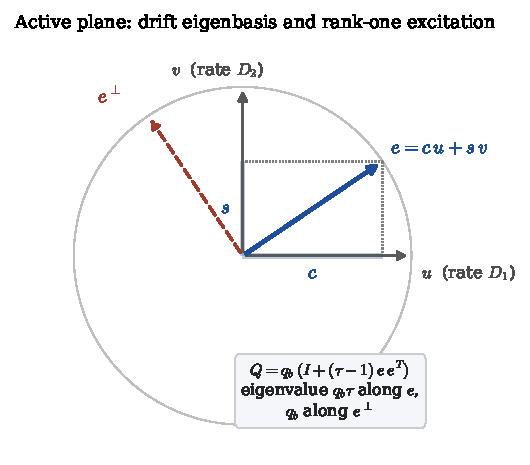
\includegraphics[width=0.52\textwidth]{figures/fig1.pdf}
\caption{The active plane. The drift is diagonal in the eigenbasis $(u,v)$ with rates
$D_1,D_2$; the forcing is isotropic except for a rank-one deformation of relative size $\tau$
along the excitation direction $e=cu+sv$. The mixing $c^2s^2$ and the rate contrast $\nu$ are the
only features of this picture that enter the determinant.}
\label{fig:plane}
\end{figure}

\section{The active covariance block}\label{sec:thm1}

\begin{theorem}[Stationary covariance on the active plane]\label{thm:cov}
Let $D_1,D_2>0$ and let $Q$ be any symmetric forcing on $\Pi$ with entries $q_{11},q_{12},q_{22}$
in the basis $(u,v)$. Then \eqref{eq:lyap} restricted to $\Pi$ has the unique solution
\begin{equation}
  \Sig = \begin{pmatrix}
    \dfrac{q_{11}}{2D_1} & \dfrac{q_{12}}{D_1+D_2}\\[2.2ex]
    \dfrac{q_{12}}{D_1+D_2} & \dfrac{q_{22}}{2D_2}
  \end{pmatrix},
  \qquad\text{that is,}\qquad
  \Sig_{ij}=\frac{Q_{ij}}{D_i+D_j}. \label{eq:modal}
\end{equation}
For the rank-one forcing \eqref{eq:forcing} this reads
\begin{equation}
  \Sig = \begin{pmatrix}
    \dfrac{q_b\bigl(1+(\tau-1)c^2\bigr)}{2D_1} & \dfrac{q_b(\tau-1)cs}{D_1+D_2}\\[2.2ex]
    \dfrac{q_b(\tau-1)cs}{D_1+D_2} & \dfrac{q_b\bigl(1+(\tau-1)s^2\bigr)}{2D_2}
  \end{pmatrix}. \label{eq:activecov}
\end{equation}
\end{theorem}

\begin{proof}
With $M|_\Pi=\operatorname{diag}(-D_1,-D_2)$, equation \eqref{eq:lyap} reads entrywise
$-(D_i+D_j)\Sig_{ij}=-Q_{ij}$, which determines each $\Sig_{ij}$ uniquely because $D_i+D_j>0$.
Substituting the entries of \eqref{eq:forcing} gives \eqref{eq:activecov}.
\end{proof}

Equation \eqref{eq:modal} is the standard modal form of the Lyapunov solution for a symmetric
drift and is used throughout the heterogeneous-OU literature
\cite{Barucca2014,GodrecheLuck2019,FerreiraMetzBarucca2025}; we claim no novelty for it. It is
recorded as a theorem only because everything below is computed from it.

\begin{lemma}[Forcing determinant]\label{lem:detQ}
For $c^2+s^2=1$, $\det Q(\tau)=q_b^2\tau$.
\end{lemma}

\begin{proof}
$Q(\tau)$ has eigenvalues $q_b\tau$ and $q_b$; equivalently, expanding the $2\times2$ determinant
of \eqref{eq:forcing} and using $c^2+s^2=1$ gives
$q_b^2\bigl[(1+(\tau-1)c^2)(1+(\tau-1)s^2)-(\tau-1)^2c^2s^2\bigr]=q_b^2\tau$.
\end{proof}

\section{Self-duality of the forcing family}\label{sec:selfdual}

The palindromic structure of the next section is not an accident of the algebra; it descends from
a symmetry of the family \eqref{eq:forcing} itself.

\begin{proposition}[Self-duality]\label{prop:selfdual}
Let $c^2+s^2=1$ and $\tau>0$. Then
\begin{equation}
  Q_e(\tau) \;=\; \tau\;Q_{\eperp}\!\left(\frac1\tau\right), \label{eq:selfdual}
\end{equation}
where $Q_{\eperp}(\sigma)=q_b\bigl(I+(\sigma-1)\eperp\eperpT\bigr)$.
\end{proposition}

\begin{proof}
Because $(e,\eperp)$ is an orthonormal basis of $\Pi$,
\begin{equation}
  ee\T+\eperp\eperpT = I. \label{eq:resolution}
\end{equation}
Hence $q_b\bigl(I+(\tau-1)ee\T\bigr)=q_b\bigl(\tau\,ee\T+\eperp\eperpT\bigr)$, and likewise
$\tau q_b\bigl(I+(\tau^{-1}-1)\eperp\eperpT\bigr)
 =\tau q_b\bigl(ee\T+\tau^{-1}\eperp\eperpT\bigr)
 =q_b\bigl(\tau ee\T+\eperp\eperpT\bigr)$.
The two agree.
\end{proof}

Equation \eqref{eq:selfdual} says that inverting the heterogeneity ratio and rotating the
excitation by a quarter turn returns the same forcing up to an overall scale $\tau$. Since the
determinant of a $2\times2$ matrix scales as $\tau^2$ under $Q\mapsto\tau Q$, and since $\Sig$
depends linearly on $Q$ by Theorem~\ref{thm:cov}, the map $\tau\mapsto1/\tau$ can only act on
$\det\Sig$ by a factor $\tau^2$ together with the exchange $c\leftrightarrow s$. The coefficient
$\Aco=c^2s^2\nu^2$ is symmetric in $c\leftrightarrow s$, which is precisely why the exchange
leaves the polynomial invariant and makes it palindromic.

\begin{remark}
Self-duality of this kind is elementary and we do not present it as a new concept; identity
\eqref{eq:resolution} is the resolution of the identity on a plane. The contribution here is its
role as the structural cause of the determinant identity in Section~\ref{sec:thm2}.
\end{remark}

\section{The palindromic determinant}\label{sec:thm2}

\begin{theorem}[Palindromic determinant identity]\label{thm:palindromic}
Let $D_1,D_2>0$, $c^2+s^2=1$, $q_b\in\Real$, $\tau\in\Real$, and let $\Sig$ be as in
\eqref{eq:activecov}. Then
\begin{equation}
  4D_1D_2\,\det\Sig
  \;=\; q_b^2\Bigl(\Aco\,\tau^2 \;+\; (1-2\Aco)\,\tau \;+\; \Aco\Bigr),
  \qquad \Aco=c^2s^2\nu^2. \label{eq:palindromic}
\end{equation}
In particular the quadratic in $\tau$ is \emph{palindromic}: its leading and constant
coefficients are equal.
\end{theorem}

\begin{proof}
Write $\Delta=D_1+D_2$. From \eqref{eq:activecov},
\[
  \det\Sig
  = \frac{q_b^2\bigl(1+(\tau-1)c^2\bigr)\bigl(1+(\tau-1)s^2\bigr)}{4D_1D_2}
    - \frac{q_b^2(\tau-1)^2c^2s^2}{\Delta^2}.
\]
Multiplying by $4D_1D_2\Delta^2$ and using Lemma~\ref{lem:detQ} in the form
$q_b^2\bigl(1+(\tau-1)c^2\bigr)\bigl(1+(\tau-1)s^2\bigr)-q_b^2(\tau-1)^2c^2s^2=q_b^2\tau$ gives
\begin{align}
  4D_1D_2\Delta^2\det\Sig
  &= \Delta^2\Bigl[q_b^2\tau + q_b^2(\tau-1)^2c^2s^2\Bigr] - 4D_1D_2\,q_b^2(\tau-1)^2c^2s^2
  \notag\\
  &= q_b^2\Bigl[\Delta^2\tau + c^2s^2(\tau-1)^2\bigl(\Delta^2-4D_1D_2\bigr)\Bigr]
  \notag\\
  &= q_b^2\Bigl[\Delta^2\tau + c^2s^2(D_1-D_2)^2(\tau-1)^2\Bigr], \label{eq:keystep}
\end{align}
since $\Delta^2-4D_1D_2=(D_1-D_2)^2$. Dividing by $\Delta^2$ and using
$\Aco=c^2s^2(D_1-D_2)^2/\Delta^2$,
\[
  4D_1D_2\det\Sig = q_b^2\bigl[\tau+\Aco(\tau-1)^2\bigr]
  = q_b^2\bigl[\Aco\tau^2+(1-2\Aco)\tau+\Aco\bigr]. \qedhere
\]
\end{proof}

Two features of \eqref{eq:keystep} deserve comment. First, the entire dependence on the rates
enters through the single combination $(D_1-D_2)^2/(D_1+D_2)^2=\nu^2$: the determinant does not
see $D_1$ and $D_2$ separately beyond the overall factor $4D_1D_2$. Second, the heterogeneity
enters only through $(\tau-1)^2$, which is manifestly symmetric under the substitution that
sends $\tau-1$ to $\tau(\tau^{-1}-1)$; this is the self-duality of
Proposition~\ref{prop:selfdual} reappearing as the palindromic symmetry of the coefficients.

\section{The reciprocal reduction}\label{sec:thm3}

Only now, with palindromicity established, do we introduce the reciprocal coordinate. A
palindromic polynomial of even degree $2m$ in $t$ is a polynomial of degree $m$ in $t+1/t$ after
division by $t^m$; for $m=1$ this is immediate, and the general statement is classical
(see \cite[\S2]{Vieira2019}, where the substitution $x=z+1/z$ and its Chebyshev connection are
set out). We use only the $m=1$ case, which we prove in line; the citation is for provenance of
the substitution, not for the identity below.

\begin{definition}
For $\tau>0$ set $w=\tau+\dfrac1\tau$.
\end{definition}

\begin{lemma}\label{lem:wge2}
For $\tau>0$, $w-2=(\tau-1)^2/\tau\ge0$, with equality if and only if $\tau=1$. Hence $w\ge2$
always, and $w=2$ exactly in the homogeneous case.
\end{lemma}

\begin{theorem}[Reciprocal reduction]\label{thm:reciprocal}
Let $D_1,D_2>0$, $c^2+s^2=1$, $q_b\ne0$, $\tau>0$. Then
\begin{equation}
  \frac{4D_1D_2\,\det\Sig}{q_b^2\,\tau}
  \;=\; 1+\Aco\,(w-2). \label{eq:normalized}
\end{equation}
\end{theorem}

\begin{proof}
Divide \eqref{eq:palindromic} by $q_b^2\tau$, which is nonzero:
\[
  \frac{\Aco\tau^2+(1-2\Aco)\tau+\Aco}{\tau}
  = \Aco\tau+1-2\Aco+\frac{\Aco}{\tau}
  = 1+\Aco\Bigl(\tau+\frac1\tau-2\Bigr). \qedhere
\]
\end{proof}

The normalization in \eqref{eq:normalized} is natural: $q_b^2\tau=\det Q$ by
Lemma~\ref{lem:detQ}, and $4D_1D_2=\prod_{i,j}(D_i+D_j)^{1/2}\cdot\ldots$ --- more simply,
$q_b^2\tau/(4D_1D_2)$ is exactly $\det\Sig$ in the homogeneous-direction case $\Aco=0$. So
\eqref{eq:normalized} compares the determinant against what it would be with no reciprocal
contribution, and the comparison is \emph{exactly affine} in $w$ (Figure~\ref{fig:affine}).

\begin{figure}[t]
\centering
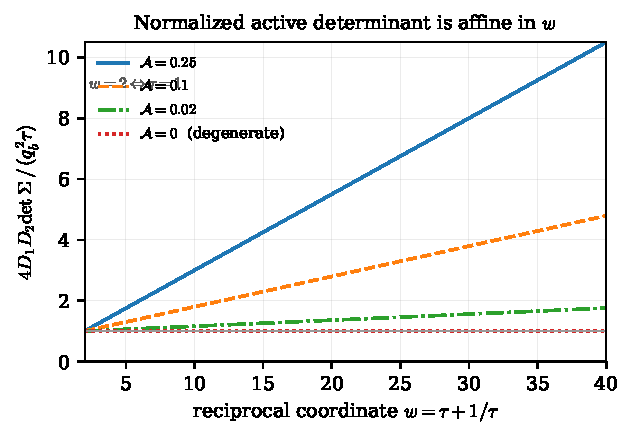
\includegraphics[width=0.66\textwidth]{figures/fig2.pdf}
\caption{The normalized active determinant \eqref{eq:normalized} as a function of the reciprocal
coordinate $w$, for several values of $\Aco$. The dependence is exactly affine, with slope
$\Aco\in[0,1/4)$ and value $1$ at $w=2$ (the homogeneous point $\tau=1$).}
\label{fig:affine}
\end{figure}

\section{Degeneracy and size of the coefficient}\label{sec:degeneracy}

Everything in \eqref{eq:normalized} is controlled by the single number $\Aco=c^2s^2\nu^2$. We
record exactly when it vanishes and how large it can be.

\begin{proposition}[Exact degeneracy conditions]\label{prop:degenerate}
Let $D_1,D_2>0$ and $c^2+s^2=1$. Then $\Aco\ge0$, and
\begin{equation}
  \Aco = 0 \iff c=0 \ \text{ or }\ s=0 \ \text{ or }\ D_1=D_2. \label{eq:degen}
\end{equation}
Separately, the reciprocal \emph{contribution} $\Aco(w-2)$ vanishes if and only if
$\Aco=0$ or $\tau=1$.
\end{proposition}

\begin{proof}
$\Aco=c^2s^2\nu^2$ is a product of squares, hence nonnegative, and vanishes iff $c=0$, $s=0$ or
$D_1-D_2=0$ (note $D_1+D_2>0$, so $\nu$ is well defined and $\nu=0$ iff $D_1=D_2$). The second
statement follows from Lemma~\ref{lem:wge2}.
\end{proof}

The three degeneracies have clean readings, and together they say exactly what the mechanism
requires:
\begin{itemize}\itemsep2pt
\item $c=0$ or $s=0$: the excitation lies in a \emph{single} drift eigenmode. The forcing is then
  simultaneously diagonalizable with the drift, the covariance is diagonal, and heterogeneity
  cannot couple the modes.
\item $D_1=D_2$: no relaxation contrast. The active block is a multiple of the identity in its
  rate structure, and the determinant is blind to how the forcing is oriented.
\item $\tau=1$: no forcing heterogeneity at all.
\end{itemize}
Thus a nonzero reciprocal contribution requires \emph{both} genuinely mixed excitation and
genuinely unequal rates. This is the sharpest explanatory content of the theorem: the effect is
an interference between two anisotropies --- one in the drift, one in the forcing --- and it
disappears if either is absent.

\begin{proposition}[Modal-mixture bound]\label{prop:mixing}
If $c^2+s^2=1$ then $c^2s^2\le\tfrac14$, with equality if and only if $c^2=s^2=\tfrac12$.
If moreover $D_1,D_2>0$ then $\nu^2<1$. Consequently
\begin{equation}
  0\;\le\;\Aco\;<\;\tfrac14. \label{eq:Abound}
\end{equation}
\end{proposition}

\begin{proof}
$\tfrac14-c^2s^2=\tfrac14-c^2(1-c^2)=(c^2-\tfrac12)^2\ge0$, with equality iff $c^2=\tfrac12$.
For the rate contrast, $(D_1+D_2)^2-(D_1-D_2)^2=4D_1D_2>0$, so $\nu^2<1$ strictly.
\end{proof}

\begin{remark}
The bound $c^2s^2\le1/4$ says the heterogeneity-sensitive coefficient is largest when the
excitation projects equally onto the two active modes. We read this as a statement about this
determinant and nothing more; it is not proposed as a physical optimality principle. Note also
that $\Aco<1/4$ is strict: $\nu^2<1$ for any finite positive rates, and $\nu^2\to1$ only in the
singular limit $D_2/D_1\to0$ or $\infty$.
\end{remark}

\section{The threshold theorem}\label{sec:threshold}

In applications the active block sits inside a larger system and one compares the determinant at
coupling $\kappa$ against a reference. Both effects --- the shrinking of the homogeneous
determinant and the reciprocal enhancement --- combine into a single scalar comparison.

\begin{theorem}[Exact threshold]\label{thm:threshold}
Let $\Phi>0$ and $C>0$ and consider
\begin{equation}
  V \;=\; \Phi\bigl(1+C\,(w-2)\bigr). \label{eq:V}
\end{equation}
Then
\begin{equation}
  V>1 \iff \Phi C\,(w-2) > 1-\Phi \iff w \;>\; w^{*}, \qquad
  w^{*} \;=\; 2+\frac{1-\Phi}{\Phi C}. \label{eq:threshold}
\end{equation}
\end{theorem}

\begin{proof}
The first equivalence is a rearrangement of \eqref{eq:V}. For the second, the identity
\[
  w-\Bigl(2+\frac{1-\Phi}{\Phi C}\Bigr) \;=\; \frac{\Phi\bigl(1+C(w-2)\bigr)-1}{\Phi C}
\]
holds identically, and $\Phi C>0$, so the left side is positive exactly when the numerator on the
right is.
\end{proof}

\begin{remark}[Edge cases, stated rather than hidden]\label{rem:edge}
Three cases deserve explicit mention.
\begin{enumerate}\itemsep2pt
\item If $\Phi\ge1$ then $w^{*}\le2$. Since $w\ge2$ always (Lemma~\ref{lem:wge2}), the threshold
  is then vacuous: the determinant already exceeds the reference at $w=2$, with no heterogeneity
  required. In the graph applications below $\Phi<1$ for $\kappa>0$, so this does not occur there,
  but the general statement must allow it.
\item If $C=0$ the equivalence \eqref{eq:threshold} is unavailable --- \eqref{eq:V} reduces to
  $V=\Phi$, independent of $w$, and no amount of heterogeneity helps. This is exactly the
  degenerate case of Proposition~\ref{prop:degenerate}.
\item $w^{*}$ is a threshold in the \emph{variance} invariant. Translating to an amplitude ratio
  requires \eqref{eq:tvsr}; failing to do so is the easiest way to misreport a constant by a
  square.
\end{enumerate}
\end{remark}

\section{Passive modes and the ambient system}\label{sec:passive}

Theorem~\ref{thm:palindromic} concerns a $2\times2$ block. We now record, as an analytic
statement, how that block sits inside an $n$-dimensional system --- and we are careful about what
is proved versus what is formalized.

\begin{proposition}[Determinant factorization]\label{prop:factor}
Let $M$ be symmetric and Hurwitz on $\Real^n$ with eigenmodes $\psi_1,\dots,\psi_n$ and rates
$D_1,\dots,D_n>0$. Suppose the forcing is
\begin{equation}
  Q = q_b\bigl(I+(\tau-1)ee\T\bigr) \label{eq:Qambient}
\end{equation}
with $e$ a unit vector whose modal support lies in $\Pi=\operatorname{span}(\psi_1,\psi_2)$, i.e.
$e=c\psi_1+s\psi_2$ with $c^2+s^2=1$. Then $\Sig$ block-diagonalizes as
$\Sig|_\Pi\oplus\Sig|_{\Pi^{\perp}}$ and
\begin{equation}
  \det\Sig \;=\; \underbrace{\frac{q_b^2\,\tau\,\bigl[1+\Aco(w-2)\bigr]}{4D_1D_2}}_{\text{active block}}
  \;\cdot\;
  \prod_{j\ge3}\frac{q_b}{2D_j}
  \;=\; \frac{q_b^{\,n}\,\tau\,\bigl[1+\Aco(w-2)\bigr]}{2^{\,n}\prod_{j=1}^{n}D_j}. \label{eq:factored}
\end{equation}
\end{proposition}

\begin{proof}
In the modal basis $Q$ has entries $\widetilde Q_{ij}=q_b\delta_{ij}+q_b(\tau-1)\tilde e_i\tilde e_j$
with $\tilde e=(c,s,0,\dots,0)$. Hence $\widetilde Q_{ij}=0$ whenever $i\le2<j$ or $j\le2<i$, so
$\widetilde Q$ is block diagonal. By \eqref{eq:modal}, $\widetilde\Sig_{ij}=\widetilde Q_{ij}/(D_i+D_j)$
inherits the same block structure, and the determinant factors. The active factor is
Theorem~\ref{thm:reciprocal}; each passive mode contributes $\widetilde\Sig_{jj}=q_b/(2D_j)$.
\end{proof}

\begin{remark}[Formalized versus documented]\label{rem:formalized}
Proposition~\ref{prop:factor} is proved here analytically. The machine-checked theorem
(Section~\ref{sec:lean}) is the \emph{explicit active block} --- Theorems~\ref{thm:cov},
\ref{thm:palindromic}, \ref{thm:reciprocal} and \ref{thm:threshold}. The general
invariant-subspace reduction of Proposition~\ref{prop:factor} is documented analytically and is
\emph{not} formalized. We are explicit about this because the distinction is easy to blur: no
claim is made that Lean verifies an arbitrary $n\times n$ invariant-subspace reduction.
\end{remark}

\subsection{Effective active dimension}\label{sec:effdim}

Proposition~\ref{prop:factor} motivates a piece of vocabulary, which we introduce with care.

The hypothesis is not that the system is two-dimensional. The ambient dimension is $n$, the
stationary law has full support on $\Real^n$, and all $n$ modes are excited --- the passive ones
simply at the baseline intensity $q_b$. What is two-dimensional is the \emph{support of the
heterogeneity}: the rank-one deformation $ (\tau-1)ee\T$ has its modal support inside $\Pi$. We
therefore say the configuration has

\begin{center}
\begin{tabular}{ll}
\toprule
ambient dimension & $n$\\
heterogeneous active dimension & $2$\\
\bottomrule
\end{tabular}
\end{center}

and we call $\Pi$ the active subspace. This is interpretation attached to a hypothesis, not a
separate theorem: nothing is claimed beyond Proposition~\ref{prop:factor}. In particular we do
\emph{not} say that the system ``is really two-dimensional''.

The point of the vocabulary is the negative result it makes sayable. If the excitation has modal
support in three or more modes, the forcing block is no longer $2\times2$, the determinant is no
longer a quadratic in $\tau$, and there is no reason for a single reciprocal coordinate to
suffice. Section~\ref{sec:obstruction} makes the corresponding spectral statement precise. The
one-coordinate closure is a feature of effective active dimension two and should not be
extrapolated.

\section{A weak-coupling law}\label{sec:weak}

Before specializing, we record a general fact about the onset of coupling which is independent of
everything above --- in particular of the two-dimensional hypothesis --- and which puts the graph
results in context.

\begin{proposition}[Weak-coupling derivative]\label{prop:weak}
Let $S$ be symmetric, $a>0$, and let $\Sig(\kappa)$ solve
$(aI+\kappa S)\Sig+\Sig(aI+\kappa S)=Q$ for a fixed positive-definite $Q$. Then
\begin{equation}
  \frac{d}{d\kappa}\Bigl[\log\det\Sig(\kappa)\Bigr]_{\kappa=0}
  \;=\; -\frac{\tr S}{a}, \label{eq:weak}
\end{equation}
independently of $Q$.
\end{proposition}

\begin{proof}
At $\kappa=0$ the equation gives $\Sig_0=Q/(2a)$. Differentiating at $\kappa=0$,
$S\Sig_0+\Sig_0S+2a\Sig'=0$, so $\Sig'=-(S\Sig_0+\Sig_0S)/(2a)$. Hence
\[
  \frac{d}{d\kappa}\log\det\Sig\Big|_0=\tr\bigl(\Sig_0^{-1}\Sig'\bigr)
  =-\frac{\tr\bigl(\Sig_0^{-1}S\Sig_0\bigr)+\tr S}{2a}
  =-\frac{2\tr S}{2a}=-\frac{\tr S}{a}. \qedhere
\]
\end{proof}

For a graph Laplacian, $\tr L=2|E|$, so \eqref{eq:weak} reads $-2|E|/a$: the initial logarithmic
rate of change of the generalized variance counts edges and is blind to the noise profile
entirely. In particular it is strictly negative, so infinitesimal coupling always contracts the
stationary covariance volume --- which is the general form of the two-node statement
$A'(0)<0$ of \cite{DeJesus2026ou}, there proved for $K_2$ only. Any enhancement, here as there,
is necessarily a finite-coupling phenomenon; this is what makes the minimization over $\kappa$ in
Section~\ref{sec:graphs} meaningful rather than vacuous.

\section{Graph corollaries}\label{sec:graphs}

We now specialize to a concrete family. Let $G$ be a connected graph on $n$ nodes with Laplacian
$L$, and take
\begin{equation}
  M = -(aI+\kappa L), \qquad a>0,\ \kappa\ge0, \label{eq:graphdrift}
\end{equation}
so the modal rates are $D_j=a+\kappa\lambda_j$ for Laplacian eigenvalues
$0=\lambda_0\le\lambda_1\le\dots\le\lambda_{n-1}$. Let the forcing be \eqref{eq:Qambient} with $e$
a node indicator: heterogeneity at a single node. Define
\begin{equation}
  \Phi(\kappa) = \prod_{j\ge1}\frac{a}{a+\kappa\lambda_j},
  \qquad
  V(\kappa,\tau) = \frac{\det\Sig(\kappa,\tau)}{\det\Sig(0,\tau)}. \label{eq:Phidef}
\end{equation}

\begin{corollary}[Graph form of the threshold]\label{cor:graph}
Suppose the node indicator $e$ has modal support in exactly two eigenmodes, with rates $D_1,D_2$
and weights $c^2,s^2$. Then
\begin{equation}
  V(\kappa,\tau) = \Phi(\kappa)\bigl[1+\Aco(\kappa)\,(w-2)\bigr],
  \qquad \Aco(\kappa)=c^2s^2\nu(\kappa)^2, \label{eq:graphV}
\end{equation}
and $V>1$ exactly when $w>w^{*}(\kappa)=2+(1-\Phi)/(\Phi\Aco)$.
\end{corollary}

\begin{proof}
By \eqref{eq:factored}, $\det\Sig(\kappa,\tau)=q_b^n\tau[1+\Aco(w-2)]/(2^n\prod_jD_j)$. At
$\kappa=0$ all rates equal $a$, so $\nu=0$, $\Aco=0$, and
$\det\Sig(0,\tau)=q_b^n\tau/(2^na^n)$. Dividing gives \eqref{eq:graphV} with
$\prod_j a/D_j=\Phi$. Theorem~\ref{thm:threshold} then applies.
\end{proof}

The optimal threshold for a given graph and forced node is
$w^{*}_{\min}=\min_{\kappa>0}w^{*}(\kappa)$: the least heterogeneity that can ever produce
enhancement, optimized over coupling strength. Figure~\ref{fig:curves} shows the three curves
computed below.

\begin{figure}[t]
\centering
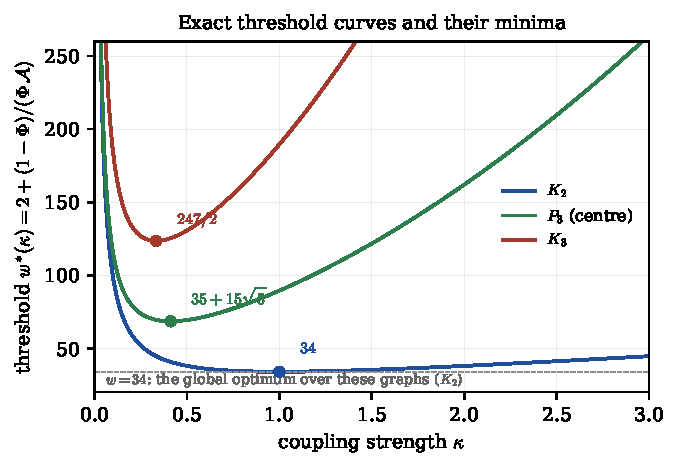
\includegraphics[width=0.70\textwidth]{figures/fig3.pdf}
\caption{Exact threshold curves $w^{*}(\kappa)$ for $K_2$, $P_3$ (centre node forced) and $K_3$,
with their exact minima marked. Each curve is the rational function derived in
Sections~\ref{sec:K2}--\ref{sec:K3}; the marked points are the exact algebraic constants, not
numerical optima.}
\label{fig:curves}
\end{figure}

\subsection{$K_2$: recovering the two-node model}\label{sec:K2}

For $K_2$ with $a=1$, the Laplacian eigenvalues are $0$ and $2$, so $D_1=1$, $D_2=1+2\kappa$, and
$\Phi=1/(1+2\kappa)$. A node indicator has weights $c^2=s^2=\tfrac12$ on the two modes, so
$c^2s^2=\tfrac14$ and
\[
  \Aco(\kappa)=\tfrac14\nu^2,\qquad \nu=\frac{1-(1+2\kappa)}{1+(1+2\kappa)}=\frac{-\kappa}{1+\kappa}.
\]
Corollary~\ref{cor:graph} gives
\begin{equation}
  V(\kappa,\tau)=\frac{1}{1+2\kappa}\left[1+\frac14\frac{\kappa^2}{(1+\kappa)^2}(w-2)\right],
  \label{eq:K2V}
\end{equation}
which is exactly the volume ratio of \cite{DeJesus2026ou} after the substitution $\tau=r^2$.
Minimizing $w^{*}(\kappa)$ over $\kappa>0$ gives
\begin{equation}
  \kappa^{*}=1,\qquad w^{*}_{\min}=34. \label{eq:K2min}
\end{equation}
By \eqref{eq:tvsr}, $w=34$ corresponds to $r+1/r=6$, i.e.\ $r=3+2\sqrt2$, which is exactly the
threshold of \cite{DeJesus2026ou}. The coupling $\kappa^{*}=1$ is the tangency at which the
enhancement window of that paper closes to a point.

\begin{remark}
This is the sense in which the two-node result is a corollary rather than a separate theorem. It
is also a check on Remark~\ref{rem:variance}: the constant $34$ is a value of $w=\tau+1/\tau$,
while $6$ is a value of $r+1/r$, and $34=6^2-2$.
\end{remark}

\subsection{$P_3$: the path on three nodes}\label{sec:P3}

For $P_3$ the Laplacian has spectrum $\{0,1,3\}$ with orthonormal eigenvectors
\[
  \psi_0=\tfrac{1}{\sqrt3}(1,1,1),\quad
  \psi_1=\tfrac{1}{\sqrt2}(1,0,-1),\quad
  \psi_2=\tfrac{1}{\sqrt6}(1,-2,1).
\]
Force the \emph{centre} node, $e=(0,1,0)$. Its modal components are
$\langle\psi_0,e\rangle=1/\sqrt3$, $\langle\psi_1,e\rangle=0$, $\langle\psi_2,e\rangle=-2/\sqrt6$.
The vanishing middle component is the crucial structural fact: \emph{the centre-node excitation
has no support on the $\lambda=1$ mode}, so its active support is exactly two-dimensional and
Proposition~\ref{prop:factor} applies with
\[
  c^2=\tfrac13\ (\lambda=0),\qquad s^2=\tfrac23\ (\lambda=3),\qquad
  D_1=1,\quad D_2=1+3\kappa,
\]
the $\lambda=1$ mode being passive. Then $\nu=-3\kappa/(2+3\kappa)$ and
\[
  \Aco(\kappa)=\tfrac13\cdot\tfrac23\cdot\frac{9\kappa^2}{(2+3\kappa)^2}
  =\frac{2\kappa^2}{(2+3\kappa)^2},
  \qquad
  \Phi(\kappa)=\frac{1}{(1+\kappa)(1+3\kappa)}.
\]
Substituting into $w^{*}=2+(1-\Phi)/(\Phi\Aco)$ and simplifying gives the exact curve
\begin{equation}
  w^{*}_{P_3}(\kappa)=\frac{27\kappa^3+72\kappa^2+64\kappa+16}{2\kappa}. \label{eq:P3curve}
\end{equation}

\begin{corollary}[$P_3$ constant]\label{cor:P3}
$\displaystyle\min_{\kappa>0}w^{*}_{P_3}(\kappa)=35+15\sqrt5$, attained at
$\kappa^{*}=\dfrac{\sqrt5-1}{3}$.
\end{corollary}

\begin{proof}
The exact factorization
\[
  27\kappa^3+72\kappa^2+64\kappa+16-\bigl(35+15\sqrt5\bigr)\cdot2\kappa
  = 9\Bigl(\kappa-\tfrac{\sqrt5-1}{3}\Bigr)^{2}\bigl(3\kappa+6+2\sqrt5\bigr)
\]
holds identically. For $\kappa>0$ the second factor is positive, so the left side is
nonnegative, giving $w^{*}_{P_3}(\kappa)\ge35+15\sqrt5$; the double root shows equality at
$\kappa^{*}=(\sqrt5-1)/3$.
\end{proof}

\subsection{$K_3$: the triangle}\label{sec:K3}

For $K_3$ the spectrum is $\{0,3,3\}$. A node indicator has $c^2=1/3$ on $\psi_0$ and the
remaining weight $2/3$ inside the \emph{degenerate} $\lambda=3$ eigenspace. Because that
eigenspace is two-dimensional with a single common rate, one may rotate within it so that one
basis vector carries the entire projection; the excitation then has support in exactly two modes
and Proposition~\ref{prop:factor} applies with $c^2=1/3$, $s^2=2/3$, $D_1=1$, $D_2=1+3\kappa$.
The third mode is passive with the same rate $1+3\kappa$. Hence $\Aco$ is as for $P_3$ while
$\Phi$ differs:
\[
  \Aco(\kappa)=\frac{2\kappa^2}{(2+3\kappa)^2},
  \qquad
  \Phi(\kappa)=\frac{1}{(1+3\kappa)^2},
\]
giving the exact curve
\begin{equation}
  w^{*}_{K_3}(\kappa)=\frac{81\kappa^3+162\kappa^2+112\kappa+24}{2\kappa}. \label{eq:K3curve}
\end{equation}

\begin{corollary}[$K_3$ constant]\label{cor:K3}
$\displaystyle\min_{\kappa>0}w^{*}_{K_3}(\kappa)=\frac{247}{2}$, attained at
$\kappa^{*}=\dfrac13$.
\end{corollary}

\begin{proof}
$81\kappa^3+162\kappa^2+112\kappa+24-\tfrac{247}{2}\cdot2\kappa
 =81\kappa^3+162\kappa^2-135\kappa+24=3(3\kappa-1)^2(3\kappa+8)$, which is nonnegative for
$\kappa>0$ and vanishes at $\kappa=1/3$.
\end{proof}

\begin{remark}[Degenerate eigenspaces]
The $K_3$ computation uses a small but real subtlety. A node indicator in $K_3$ is not supported
on two \emph{eigenvectors} for any fixed choice of basis; it is supported on $\psi_0$ and on a
two-dimensional eigenspace. The hypothesis of Proposition~\ref{prop:factor} is nevertheless met,
because within a degenerate eigenspace any orthonormal basis is admissible and one may choose it
adapted to the projection. Where the relevant eigenvalues are \emph{distinct}, as in $P_3$, no
such freedom exists and the vanishing of a modal component is a genuine constraint.
\end{remark}

\subsection{Summary of the corollaries}

\begin{table}[t]
\centering
\caption{The three worked graph corollaries. All constants are exact and derived from
Corollary~\ref{cor:graph}; none is fitted. ``Formalized'' refers to the Lean development of
Section~\ref{sec:lean}.}
\label{tab:corollaries}
\begin{tabular}{llllll}
\toprule
Model & Active rates & $c^2,s^2$ & $\kappa^{*}$ & $w^{*}_{\min}$ & Formalized\\
\midrule
$K_2$ & $1,\ 1+2\kappa$ & $\tfrac12,\tfrac12$ & $1$ & $34$ & yes\\
$P_3$ (centre) & $1,\ 1+3\kappa$ & $\tfrac13,\tfrac23$ & $\dfrac{\sqrt5-1}{3}$ & $35+15\sqrt5$ & yes\\
$K_3$ (any node) & $1,\ 1+3\kappa$ & $\tfrac13,\tfrac23$ & $\dfrac13$ & $\dfrac{247}{2}$ & yes\\
\bottomrule
\end{tabular}
\end{table}

Table~\ref{tab:corollaries} collects the results. Numerically $35+15\sqrt5\approx68.54$ and
$247/2=123.5$, both larger than the $K_2$ value $34$: among these three configurations, the
two-node system is the one for which the least heterogeneity suffices. We deliberately stop at
three worked cases rather than cataloguing families of graphs; see Section~\ref{sec:limits} for
what we do \emph{not} claim about general graphs.

\section{Two-dimensional spectral closure}\label{sec:closure}

A separate two-dimensional phenomenon explains why an earlier spectral argument closed with a
single scalar. For a positive-definite $2\times2$ matrix with eigenvalues $\mu_1\ge\mu_2>0$,
write $q=\mu_1/\mu_2\ge1$ and
\begin{equation}
  J_2(\Sig)=\frac{(\tr\Sig)^2}{\det\Sig}. \label{eq:J2}
\end{equation}

\begin{proposition}\label{prop:J2}
$J_2=q+\dfrac1q+2$, and $q\mapsto q+1/q$ is strictly increasing on $[1,\infty)$. Hence $J_2$
determines $q$ uniquely.
\end{proposition}

\begin{proof}
$(\mu_1+\mu_2)^2/(\mu_1\mu_2)=\mu_1/\mu_2+\mu_2/\mu_1+2$. Strict monotonicity of $q+1/q$ on
$[1,\infty)$ is elementary.
\end{proof}

This is standard. Scale-free trace/determinant functionals of a covariance matrix are the
classical sphericity diagnostics, going back to Mauchly \cite{Mauchly1940} and treated
textbook-style by Muirhead \cite[Ch.~8]{Muirhead1982}; trace/determinant eigenvalue bounds of this
type are likewise classical \cite{WolkowiczStyan1980,HornJohnson2012}. We claim no novelty. It is recorded because
it is the reason a single scale-free scalar suffices in dimension two --- the same reason, in a
different guise, that one reciprocal coordinate suffices in Theorem~\ref{thm:reciprocal}.

\subsection{Failure in higher dimension}\label{sec:obstruction}

\begin{proposition}[Non-identifiability for $n\ge3$]\label{prop:obstruction}
For $n=3$ the pair $(\tr\Sig,\det\Sig)$ does not determine the spectral shape: the positive
triples $(1,8,12)$ and $(2,3,16)$ have the same trace $21$ and the same determinant $96$, hence
the same value of every scale-free invariant built from trace and determinant alone, but
different extreme-eigenvalue ratios $12$ and $8$.
\end{proposition}

This too is background mathematics, not a new theorem. By Newton's identities a spectrum is
determined by all $n$ elementary symmetric functions, of which trace and determinant are the
complete list only when $n=2$; the failure above is the elementary consequence. The invariant
theory behind such statements is classical, and the statistical form is Mauchly's
\cite{Mauchly1940,Muirhead1982}.

We stress the relation to Section~\ref{sec:effdim}. Proposition~\ref{prop:obstruction} is about
the \emph{spectrum} of an $n\times n$ covariance; Proposition~\ref{prop:factor} is about the
\emph{support of the heterogeneity}. They are different statements, but they point the same way:
the one-coordinate closure used throughout this paper is a two-dimensional phenomenon. If the
excitation genuinely spans three or more modes with distinct rates, neither the palindromic
determinant nor the spectral closure is available, and we make no claim about that case.

\section{Relation to existing work, and what we claim}\label{sec:priorart}

\paragraph{Standard ingredients.} The following are classical and are used as such: the
stationary OU covariance and the Lyapunov equation \cite{Gardiner2004,Vatiwutipong2019,Simoncini2016};
the modal solution \eqref{eq:modal} for symmetric drift, standard in heterogeneous-OU work
\cite{Barucca2014,GodrecheLuck2019,FerreiraMetzBarucca2025}; the determinant as Wilks's
generalized variance \cite{Wilks1932} and its entropy reading \cite{CoverThomas2005}; graph
Laplacian eigenmodes and their use in network dynamics \cite{BamiehEtAl2012}; the reduction of a
self-reciprocal polynomial through $t+1/t$ \cite{Vieira2019}; the trace/determinant shape
statistic \cite{Mauchly1940,Muirhead1982,WolkowiczStyan1980,HornJohnson2012}.

\paragraph{Closest located prior art.} The nearest genuine antecedent is the work of Summers,
Cortesi and Lygeros on submodularity and controllability in complex networks
\cite{SummersEtAl2016}, which proves that $\log\det$ of the controllability Gramian is a monotone
increasing and submodular \emph{set} function of the chosen input columns (see also
\cite{Antoulas2005}). That is the qualitative predecessor of the present result, and it differs in
four ways that matter: it concerns a controllability Gramian rather than the stationary covariance
solving \eqref{eq:lyap}; it is a set function over discrete input subsets rather than a continuous
one-parameter family; the forcing is \emph{added} with no baseline constraint, whereas
\eqref{eq:forcing} reshapes a fixed isotropic baseline; and it yields no closed form, no
palindromic structure and no threshold. We are sharpening a qualitative monotonicity statement
into an exact identity in a narrower setting, not contradicting or subsuming it.

Two-temperature linear Langevin systems
\cite{GodrecheLuck2019,FilligerReimann2007,DotsenkoEtAl2013} share the model class exactly --- in
particular \cite[\S2.10]{GodrecheLuck2019} gives the explicit $2\times2$ stationary covariance for
arbitrary friction and diffusion --- but their scalar diagnostics are entropy production,
irreversibility and heat flux, not the covariance determinant. Likewise
\cite{BoffiDeGregorio2024} analyses precisely the two-degree-of-freedom two-temperature geometry
studied here and tracks an individual variance entry rather than the generalized variance. Low-rank
structure in Lyapunov solutions is well studied
\cite{Simoncini2016,TownsendWilber2018}, but for solution approximation and singular-value bounds
rather than determinants.

\paragraph{What we claim.} Conservatively: we did not identify, in the literature we searched, an
equivalent closed-form statement of the palindromic determinant identity
\eqref{eq:palindromic}, of its reciprocal reduction \eqref{eq:normalized}, or of the resulting
exact generalized-variance threshold optimized over a coupling parameter. We describe this as an
\emph{apparently distinct assembly of standard ingredients} and make no priority claim. Each
individual ingredient is standard, and we have cited it as such. Should an equivalent theorem
exist, the appropriate reading of this paper is as an exact derivation and machine-checked
formalization of it, not as a new result.

\paragraph{Relation to the author's other work.} The two-node model of \cite{DeJesus2026ou} is
recovered in Section~\ref{sec:K2} as the corollary $\tau=r^2$, $c^2=s^2=1/2$; that paper is the
motivating special case and is cited rather than reproduced. Separately, \cite{DeJesus2026dual}
records a reciprocal invariant $\tr(T)\tr(T^{-1})$ determining a two-dimensional shape ratio up
to inversion, and is relevant as conceptual background on one-coordinate completeness in two
dimensions. We state explicitly that the present theorem is derived independently from Lyapunov
covariance dynamics; \cite{DeJesus2026dual} is invariant-theoretic context, not a source for it.

\section{Limitations}\label{sec:limits}

\begin{enumerate}\itemsep3pt
\item The results are exact statements about a linear-Gaussian model. No nonlinear, biological,
  cognitive, social or physical-universality claim is made or implied, and no significance is
  attached to the numerical values of the constants beyond this model class.
\item Theorems~\ref{thm:cov}--\ref{thm:threshold} require an \emph{exactly} two-dimensional
  active support. If the excitation has modal support in three or more modes with distinct rates,
  the determinant is not a quadratic in $\tau$ and nothing here applies.
\item The forcing baseline is isotropic \emph{on the active plane}. A non-isotropic baseline
  breaks the self-duality of Proposition~\ref{prop:selfdual} and with it the palindromic
  structure.
\item The drift is assumed symmetric on the active plane. Non-normal drift is outside the scope
  of the modal formula \eqref{eq:modal}.
\item Proposition~\ref{prop:factor} --- the $n$-dimensional reduction --- is proved analytically
  but is \emph{not} machine-checked. Only the $2\times2$ active block is formalized
  (Remark~\ref{rem:formalized}).
\item The formalization verifies algebra, not stochastic-process theory. That the $\Sig$ of
  \eqref{eq:lyap} is the stationary covariance of \eqref{eq:sde} is classical and is assumed, not
  verified in Lean.
\item ``Effective active dimension'' (Section~\ref{sec:effdim}) is interpretive vocabulary
  attached to a hypothesis, not an independent theorem.
\item We work out three graph corollaries. We do \emph{not} claim a general characterization of
  which graphs and forced nodes satisfy the two-dimensional active-support hypothesis, nor a
  general lower bound on $w^{*}_{\min}$ over all graphs. A bound of that kind was explored in
  preparatory work but is not reproduced here, because we were not able to reconstruct its proof
  to the standard applied elsewhere in this paper; see Section~\ref{sec:open}.
\item Optimizing $w^{*}$ over $\kappa$ treats coupling as freely tunable and the forcing
  geometry as fixed. Other optimizations are possible and would give different constants.
\end{enumerate}

\section{Machine-checked verification}\label{sec:lean}

The central algebraic content is formalized in Lean~4 with mathlib, in the public repository
\url{https://github.com/innerlightr-wq/ou-threshold-lean}. Within it:

\begingroup\small\raggedright
\begin{itemize}\itemsep2pt
\item the results of this paper live in \texttt{OUCorridor/ActivePlane.lean} and
  \texttt{OUCorridor/SpectralShape.lean};
\item supporting material is in \texttt{Covariance.lean}, \texttt{Threshold.lean},
  \texttt{MainTheorem.lean}, \texttt{ResidualThreshold.lean} and \texttt{CrossThreshold.lean};
\item a frozen snapshot of the exact sources, environment and build is kept at
  \texttt{verified/active-plane-2026-09/}.
\end{itemize}
\endgroup

\begin{table}[t]
\centering
\caption{Correspondence between the statements of this paper and the machine-checked theorems.}
\label{tab:lean}
\small
\begin{tabular}{@{}l p{0.50\textwidth} l@{}}
\toprule
This paper & Lean name & Status\\
\midrule
Theorem~\ref{thm:cov} & \texttt{activeCov\_lyapunov}, \texttt{activeCov\_unique} & formalized\\
Lemma~\ref{lem:detQ} & \texttt{det\_activeForcing} & formalized\\
Proposition~\ref{prop:selfdual} & \texttt{activeForcing\_self\_dual} & formalized\\
Theorem~\ref{thm:palindromic} & \texttt{det\_activeCov\_palindromic} & formalized\\
Lemma~\ref{lem:wge2} & \texttt{two\_le\_reciprocalExcitation}, \texttt{reciprocalExcitation\_eq\_two\_iff} & formalized\\
Theorem~\ref{thm:reciprocal} & \texttt{normalizedActiveDet\_eq} & formalized\\
Proposition~\ref{prop:degenerate} & \texttt{activeCoeff\_eq\_zero\_iff} & formalized\\
Proposition~\ref{prop:mixing} & \texttt{mixing\_le\_quarter}, \texttt{rateContrast\_sq\_lt\_one} & formalized\\
Theorem~\ref{thm:threshold} & \texttt{volumeRatio\_gt\_one\_iff} & formalized\\
Section~\ref{sec:K2} & \texttt{volume\_div\_volume0\_eq}, \texttt{reciprocalExcitation\_sq} & formalized\\
Corollary~\ref{cor:P3} & \texttt{p3\_thresholdCurve\_eq}, \texttt{p3\_threshold\_min/\_attained} & formalized\\
Corollary~\ref{cor:K3} & \texttt{k3\_thresholdCurve\_eq}, \texttt{k3\_threshold\_min/\_attained} & formalized\\
Proposition~\ref{prop:J2} & \texttt{J2\_eq\_reciprocalInvariant}, \texttt{eigen\_ratio\_unique\_of\_J2} & formalized\\
Proposition~\ref{prop:obstruction} & \texttt{exists\_same\_trace\_det\_different\_ratio} & formalized\\
\midrule
Proposition~\ref{prop:factor} & --- & analytic only\\
Section~\ref{sec:effdim} & --- & interpretation\\
\bottomrule
\end{tabular}
\end{table}

\paragraph{Environment.} Lean 4.33.1 (\texttt{x86\_64-unknown-linux-gnu}), with mathlib pinned at
revision
\begin{center}
\texttt{0df444a360eaa60ab8c11dca51a86af692955474}.
\end{center}
The recorded build completes with $8715$ jobs.

\paragraph{Audit.} A grep of the library for \texttt{sorry}, \texttt{admit} and \texttt{axiom}
returns no matches. All $28$ audited theorems --- the $22$ of \texttt{ActivePlane.lean} and
\texttt{SpectralShape.lean} together with the pre-existing main theorems --- report exactly the
three standard axioms of mathlib's classical foundation under \texttt{\#print axioms}:
\texttt{propext}, \texttt{Classical.choice}, \texttt{Quot.sound}. There is no custom axiom and no
\texttt{sorryAx}.

\paragraph{What is not formalized.} As stated in Remark~\ref{rem:formalized} and
Table~\ref{tab:lean}: the $n$-dimensional factorization of Proposition~\ref{prop:factor}, the
interpretive content of Section~\ref{sec:effdim}, and all stochastic-process theory. Lean checks
exact real algebra on matrices. The modelling step --- that \eqref{eq:lyap} describes the
stationary covariance of \eqref{eq:sde} --- is classical and assumed.

\section{Reproducibility}\label{sec:repro}

The manuscript directory \texttt{paper/active-plane-theorem/} is self-contained: it holds
\texttt{main.tex}, its own copy of \texttt{references.bib}, the figures, the build script, the
build log, and \texttt{manuscript\_checks.py}. Every displayed identity in this paper is
re-derived and verified symbolically by that script using exact arithmetic (SymPy), with no
floating-point step in any claim: it solves the Lyapunov equation from scratch rather than
checking a pre-written solution, extracts the determinant's coefficients in $\tau$ and compares
leading against constant, derives $\Phi$ and $\Aco$ for $P_3$ and $K_3$ from the graph
Laplacians, and confirms each exact minimum by algebraic factorization. The script reports
$55/55$ checks passing.

Exact commit hashes, the branch name and file digests are recorded in the accompanying
\texttt{README.md} and \texttt{SHA256SUMS.txt} at the state in which this draft was built.

\section*{Acknowledgments}
\addcontentsline{toc}{section}{Acknowledgments}

AI-assisted tools were used for symbolic checking, literature organization and citation
verification, code support, construction and checking of the Lean development, and editorial
assistance. Claims identified in Table~\ref{tab:lean} as formalized were checked by Lean's kernel
under the pinned environment recorded in Section~\ref{sec:lean}, which does not depend on the
assistant's correctness; the remaining claims were verified symbolically by the reproducibility
script. The author reviewed the manuscript and takes responsibility for it. This draft has not
undergone independent human peer review.

\appendix

\section{Open items}\label{sec:open}

Recorded so that the gaps are explicit rather than silent.

\begin{enumerate}\itemsep3pt
\item \textbf{A general graph lower bound.} Preparatory work suggested
  \begin{equation}
    w^{*}_{\min}\;\ge\;2+\frac{64|E|}{\lambda}\;\ge\;34, \label{eq:graphbound}
  \end{equation}
  with equality only for $K_2$. The inequality chain behind it is elementary and we were able to
  reconstruct it: it combines $c^2s^2\le\tfrac14$ (Proposition~\ref{prop:mixing}), the AM--GM
  bound $(2a+\kappa\lambda)^2\ge8a\kappa\lambda$, and
  $\Phi^{-1}-1=\prod_{j\ge1}(1+\kappa\lambda_j/a)-1\ge\kappa\,\tr L/a$, each holding pointwise in
  $\kappa$ and hence surviving the minimization, together with $\tr L=2|E|$ and
  $\lambda\le\tr L$.

  It is nevertheless excluded from the body, because stating it correctly requires four
  qualifications that are easy to lose and that we did not want to carry:
  \begin{enumerate}\itemsep2pt
  \item[(a)] $\lambda$ is the Laplacian eigenvalue of the \emph{single relative eigenmode excited
    by $e$} --- the one giving $D_2=a+\kappa\lambda$. It is not the algebraic connectivity and not
    $\lambda_{\max}$. Read loosely, \eqref{eq:graphbound} becomes a different and unproved claim.
  \item[(b)] $|E|=\tfrac12\tr L$ is an unweighted edge count; for a weighted Laplacian it must be
    read as total edge weight.
  \item[(c)] The quantifier must be ``over connected graphs \emph{and admissible rank-one
    excitations}'', where admissible means the excitation has modal support in exactly two
    eigenmodes. That hypothesis genuinely fails for some graphs and nodes, and without it there is
    no $w^{*}$ to bound.
  \item[(d)] The derivation assumes the active plane \emph{contains the common mode}
    ($D_1=a$). Theorem~\ref{thm:palindromic} permits an active plane spanned by two nonzero-$\lambda$
    modes, and \eqref{eq:graphbound} as derived does not cover that case.
  \end{enumerate}
  The ``equality iff $K_2$'' direction also needs writing out rather than asserting: for a
  connected graph with $n\ge3$ the third inequality is strict for every $\kappa>0$, whence
  $w^{*}_{\min}>34$. Finally the bound is quantitatively weak away from $K_2$ (it gives $44.67$ for
  $P_3$ against the true $68.54$, and $66$ for $K_3$ against $123.5$), so its only real content is
  the corollary that $34$ is a global minimum attained only by $K_2$. Nothing above depends on it.
\item \textbf{Characterizing admissible configurations.} Which pairs (graph, forced node) give a
  node indicator with modal support in exactly two eigenmodes? The $P_3$ centre node works because
  of a symmetry-induced vanishing; $K_3$ works because of eigenvalue degeneracy. A general
  criterion is open, and is a question about graph symmetry rather than about the present theorem.
\item \textbf{Beyond rank one.} For a rank-$k$ deformation with $k\ge2$, or an excitation spanning
  three or more distinct-rate modes, the determinant is a polynomial of higher degree in the
  heterogeneity parameters and no single reciprocal coordinate is expected to suffice. We have not
  investigated whether a weaker structured reduction survives.
\item \textbf{Non-normal drift.} The modal formula \eqref{eq:modal} assumes a symmetric drift on
  the active plane. The non-normal case is open here.
\end{enumerate}

\bibliographystyle{plain}
\bibliography{references}

\end{document}
